\setchapterpreamble[u]{\margintoc}
\chapter{Equazioni differenziali ordinarie}
\labch{odes}

\section{Introduzione}

Un'equazione differenziale ordinaria (ODE) è un'equazione differenziale che
dipende da una sola variabile indipendente, \(x\). Le sue incognite consistono
in una o più funzioni \(y(x)\) e coinvolgono le derivate di queste funzioni.
Consideriamo l'equazione esplicita del primo ordine:

\[
	y' = f(x, y),
\]

La soluzione per ODE di ordine superiore può essere ottenuta trasformandole in
un sistema di ODE di primo ordine.

In generale, possiamo quindi risolvere un sistema di $n$ equazioni differenziali
al primo ordine:

\[
	\begin{cases}
		y_1'(x) = f_1(x, y_1, \dots, y_n), \quad y_1(0) = a_1 \\
		\vdots                                                \\
		y_n'(x) = f_n(x, y_1, \dots, y_n), \quad y_n(0) = a_n
	\end{cases}
	\rightarrow \mathbf{y}' = \mathbf{f}(x, \mathbf{y})
\]

\subsection{Metodi numerici}

I metodi studiati durante il corso vengono denominati \textit{a singolo passo}:
la soluzione numerica viene calcolata con il seguente approccio:

$$
	y_{n, i+1} = y_{n, i} + h \Phi(\mathbf{y}, x; h; \mathbf{f})
$$

Dove $n$ indica la coordinata di $\mathbf{y}$ e $i$ il numero del passo, e $\Phi$
è un funzionale.

Si può tradurre in C++ il funzionale $\Phi$ in un oggetto di tipo
\texttt{std::function} e successivamente si può implementare il metodo di
risoluzione generale a singolo passo nel seguente modo:

\begin{lstlisting} [language=C++] 
  ... // Dichiarazione funzione 

  // Vettore delle conditioni iniziali
  Tensor<T> y = initial\_conds\_;

  // Allocazione del tensore risultante
  Tensor<T> result =
      Tensor<T>::Matrix(
                    coords_range_.Nodes().size(),
                    initial_conds_.Rows()
      );

  // Si sceglie il funzionale in base al metodo scelto
  auto method_func = GetMethodFunction(method_);

  int step_index = 0;

  for (const auto &t : coords_range_) {
    // Si aggiunge alla riga specificata lo stato
    // precedente/iniziale del sistema
    for (int i = 0; i < y.Rows(); ++i) {
      result(step_index, i) = y(i);
    }

    // Si calcola lo stato successivo 
    y = y + method_func(t, y) * coords_range_.Step();

    step_index++;
  }

  return result;
\end{lstlisting}

\texttt{result} è una matrice con entrate
\begin{align*}
	R_{ij} & = y_j(t_i)                                                        \\
	       & i \in \left\{n \in \mathbb{N} : t_0 \leq t_n \leq t_{max}\right\} \\
	       & j \in [0, \dim{\mathcal{Y}}] \quad \mathbf{y} \in \mathcal{Y}
\end{align*}


\paragraph{Metodo di Eulero}
La procedura consiste nell'osservare che \(f(x, y(x))\) è uguale alla pendenza
\(y'(x)\) della soluzione. L'idea di base è di discretizzare la derivata con una
differenza finita, scegliendo un \(h \neq 0\) piccolo in modo tale che:

\[
	y(x + h) = y(x) + h f(x, y(x)) + O(h^2).
\]

Allora, troncando ordini quadratici, otteniamo che

\[
	\Phi = f(x, y(x))
\]

\paragraph{Metodo RK2 ed RK4}
Per ottenere metodi di ordine superiore, si deve costruire una funzione \(\Phi(x, y; h; f)\) che approssimi meglio la serie di Taylor di \(\Delta(x, y; h; f)\). Per esempio, possiamo partire con:

\begin{equation}
	\label{eq_phi}
	\Phi(x, y; h; f) = a_1 f(x, y) + a_2 f(x + p_1 h, y + p_2 h f(x, y)),
\end{equation}

Espandendo $n$ volte $\Phi$ dove $\Phi$ è stato generalizzato espandendo
ricorsivamente il ragionamento in \ref{eq_phi} si confrontano poi i
coefficienti con l'espansione di taylor di $y$ e si ottengono dei vincoli su
di essi, non unici.

Utilizzando questo ragionamento si possono ottenere, scegliendo arbitrariamente
i coefficienti liberi:
\begin{itemize}

	\item[RK2] dove il procedimento per il calcolo è:
		\[
			\begin{cases}
				k_1 = f(x, y), \\
				\Phi = f(x + \frac{1}{2} h, y + \frac{1}{2} h k_1),
			\end{cases}
		\]

	\item[RK4] dove il procedimento per il calcolo è:
		\[
			\begin{cases}
				k_1 = f(x, y),                                                \\
				k_2 = f\left(x + \frac{1}{2} h, y + \frac{1}{2} h k_1\right), \\
				k_3 = f\left(x + \frac{1}{2} h, y + \frac{1}{2} h k_2\right), \\
				\Phi = f(x + h, y + h k_3),
			\end{cases}
		\]
\end{itemize}

\section{Implementazione preliminaria}

\paragraph{Classe \texttt{ODESolver}} La classe \texttt{ODESolver} ha lo scopo di
risolvere un qualsiasi sistema di equazioni differenziali al primo ordine.

L'approccio generale in tutti gli esercizi sarà quello di inizializzare tutti i
componenti necessari per l'approssimazione numerica, inserirli nell'oggetto
\texttt{ODESolverBuilder} per costruire l'oggetto \texttt{ODESolver} e risolvere
il sistema attravero metodo \texttt{Solve()} citato nella sezione
precedente:

\begin{enumerate}
	\item Viene fornita una funzione di tipo \texttt{ode::Function<T>} la quale
	      rappresenta il sistema di equazioni differenziali.

	      \textit{Esempio}: Una particella carica in un campo elettrostatico
	      uniforme monodimensionale sarà descritta dall'equazione differenziale:
	      \[
		      \begin{cases}
			      \dot{x} = v \\
			      \dot{v} = \frac{q}{m} E
		      \end{cases}
	      \]

	      La funzione di tipo \texttt{ode::Function<T>} sarà:
	      \begin{lstlisting} [language=C++]
            // Tempo
auto f = [](T t, 
           // Condizioni al tempo t 
           Tensor<T> const& y) {
    // const T q = ..., m = ..., E = ...

    auto y_next = tensor::Tensor<double>::Vector(2);

    // dx/dt
    y_next(0) = y(1);
    // dv/dt 
    y_next(1) = q / m * E;

    return y_next;
};
        \end{lstlisting}

	\item Vengono scelte le condizioni iniziali e immagazzinate in un oggetto di
	      tipo \texttt{tensor::Tensor<T>}.

	\item Viene scelto l'intervallo di tempo e lo step utilizzato (si dichiara
	      un oggetto di tipo \texttt{func::Range<T>} di tipo \texttt{kFixed})

	\item Si sceglie il metodo numerico da utilizzare

	\item Si risolve numericamente l'equazione differenziale chiamando il metodo
	      \texttt{Solve()} ottenendo la matrice \texttt{result}.





\end{enumerate}

\section{Esercizi}

\subsection{Oscillatore approssimato}

\paragraph{Richiesta}

Risolvere l'equazione differenziale dell'oscillatore armonico con i seguenti valori iniziali:

\begin{equation}
	\ddot{\theta}(t) = -\theta(t)
\end{equation}
con $\theta(0) = 0$ e $\dot{\theta}(0) = 1$.

\begin{enumerate}
	\item Utilizzare il metodo di Eulero, il metodo di Runge-Kutta del secondo ordine (RK2) e il metodo di Runge-Kutta del quarto ordine (RK4).

	\item Ottenere la soluzione analitica $\theta(t)$ e confrontarla con la soluzione numerica $\eta(t;h)$ ottenuta con i tre metodi. Studiare l'errore:
	      \[
		      e(t,h) = \eta(t,h) - \theta(t)
	      \]
	      in funzione del passo $h$ e verificare che i metodi abbiano l'ordine atteso.

\end{enumerate}

\paragraph{Osservazioni e analisi risultati}

\begin{enumerate}
	\item Risolvendo l'esercizio secondo il ragionamento citato in 5.2 %FIXME
	      si ottengono i grafici \ref{fig:sin_comparison} e
	      \ref{fig:arcsin_comparison}. \\
	      Come si può notare il metodo di Eulero è
	      già incoerente con il dominio dell'immagine della funzione $\sin(x)$
	      per valori in $x \in (2\pi, 4\pi)$ mentre i metodi di ordine successivo  sono molto più precisi già a valori bassi di $x$ e di $h$.

	      \begin{marginfigure}
		      \hspace*{-2cm}
		      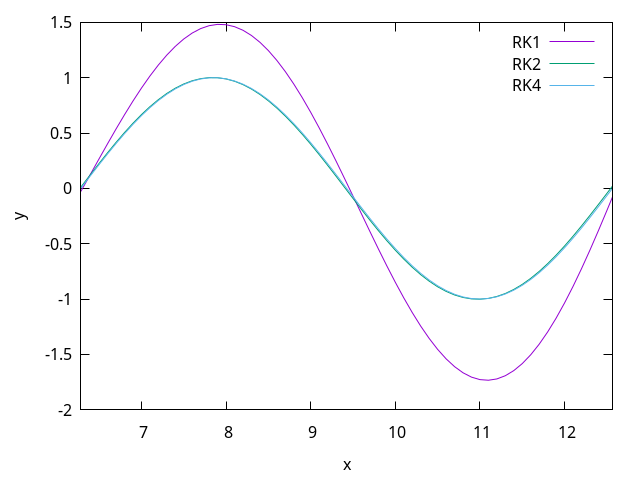
\includegraphics[width=1.5\textwidth]{oscillator_comparison.png}
		      \caption{Confronto tra soluzioni numeriche con step $h=0.1$}
		      \label{fig:sin_comparison}
		      \labfig{expfunc}
	      \end{marginfigure}

	      \begin{marginfigure}
		      \hspace*{-2cm}
		      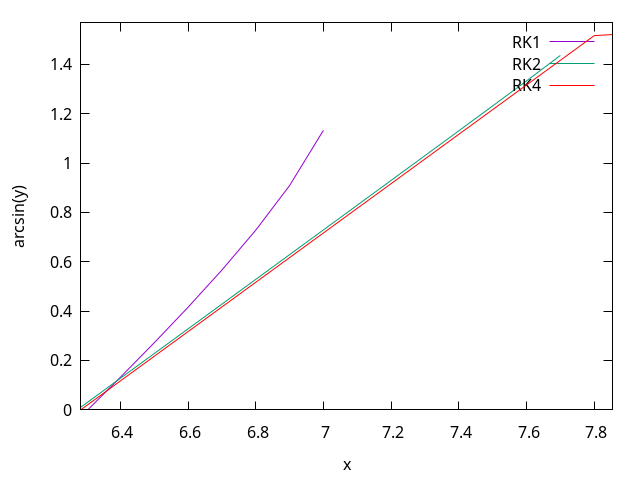
\includegraphics[width=1.5\textwidth]{arcsin_comparison.png}
		      \caption{Visualizzazione alternativa per le soluzioni numeriche
			      (step $h=0.1$)}
		      \label{fig:arcsin_comparison}
		      \labfig{expfunc}
	      \end{marginfigure}

	\item La risoluzione analitica è immediata:
	      \begin{align*}
		      \theta(t) & = Ae^{\lambda t} \rightarrow \lambda^2 + 1 = 0 \\
		      \theta(t) & = Ae^{it} + Be^{-it}                           \\
	      \end{align*}
	      \[
		      \begin{cases}
			      \theta(0) = 0 \\
			      \dot{\theta(0)} = 1
		      \end{cases}
		      \Rightarrow
		      \begin{cases}
			      A+B=0 \\
			      Ai-Bi = 1
		      \end{cases}
		      \Rightarrow
		      \theta(t) = \sin(t)
	      \]

	      Un modo per studiare l'errore è quello di valutare la
	      differenza $\eta(t_{max}, h) - \theta(t_{max})$ (poichè l'effetto di
	      propagazione dell'errore sulla approssimazione è massimo per $t_{max}$). \\
	      Campionando $(e(t_{max}, h_i), h_i)$ si ottiene la figura
	      \ref{fig:error_comparison} si può notare che, come dettato dalla
	      teoria, il metodo RK1 scala come $h$, RK2 come ${h}^2$ e RK4 come $h^{4}$.

	      \begin{marginfigure}
		      \hspace*{-2cm}
		      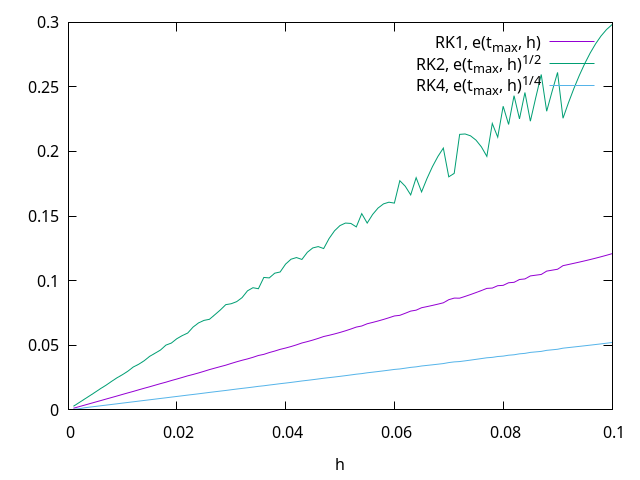
\includegraphics[width=1.5\textwidth]{ode_error_comparison.png}
		      \caption{Associando alla funzione $e(t_{max}, h)$ l'inverso della
			      funzione teoricamente associata si ottiene una relazione di
			      proporzionalità diretta tra le funzioni inverse e $h$}
		      \label{fig:error_comparison}
		      \labfig{expfunc}
	      \end{marginfigure}




	      %TODO: analisi errore, come possiamo valutare e confrontare gli 
	      % ordini?l

	      %% TODO: ulteriori metodi potrebbero essere la media quadratica
\end{enumerate}



\subsection{Oscillatore reale}

\paragraph{Richiesta}

Considerare l'equazione differenziale del pendolo senza l'approssimazione delle piccole oscillazioni:

\begin{equation}
	\ddot{\theta}(t) = -\sin{\theta(t)}
\end{equation}
con $\theta(0) = 0$ e $\dot{\theta}(0) = 1$.

\begin{enumerate}
	\item Risolvere numericamente l'equazione differenziale e tracciare il grafico di $\theta(t)$ e $\dot{\theta}(t)$ e $\dot{\theta}({\theta})$.
	\item Ripetere l'esercizio includendo un termine di attrito:
	      \[
		      \ddot{\theta}(t) = -\sin{\theta(t)} - \gamma \dot{\theta}(t)
	      \]
	\item e un termine forzante:
	      \[
		      \ddot{\theta}(t) = -\sin{\theta(t)} - \gamma \dot{\theta}(t) + A \sin{\frac{2}{3}t}
	      \]
	      con $\gamma \in (0, 2)$ e $A \in (0, 2)$.

\end{enumerate}

\paragraph{Implementazione}

\subparagraph{File necessari} \texttt{damped\_oscillator.cpp}

L'implmentazione necessita solamente di scrivere il sistema di equazioni differenziali, di seguito e' proposta l'implementazione del terzo punto:

\begin{lstlisting} [language=C++]
tensor::Tensor<double> ForcedOscillator(double t,
                                        tensor::Tensor<double> const &y) {
  auto dydt = tensor::Tensor<double>::Vector(2);

  // Dividiamo l'equazione differenziale di secondo ordine 
  // in due di primo ordine
  dydt(0) = y(1);

  // Le costanti vengono passate globalmente
  dydt(1) = -sin(y(0)) - kGamma * y(1) + kA * sin((2.0 / 3) * t);

  return dydt;
}
\end{lstlisting}

\paragraph{Osservazioni e analisi risultati}

\begin{enumerate}

	\item Si ottengono i seguenti risultati per il primo punto, si utilizza inoltre, per limitare i plot ottenuti, che il metodo utilizzato sia \textit{RK4}:

	      \begin{figure} [H]
		      \centering
		      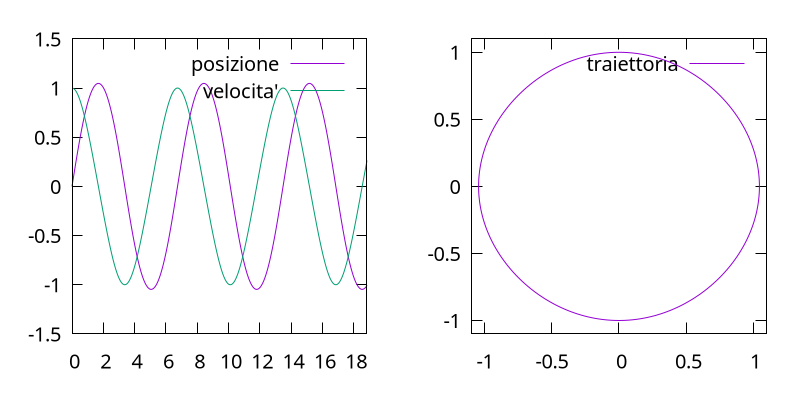
\includegraphics[width=1\textwidth]{real_oscillator_1.png}
		      \caption{Oscillatore ideale imperturbato $(\theta(0)=0, \dot{\theta}(0)=1)$, nel caso di equilibrio stabile. Nella prima figura si possono osservare $\theta(t), \dot{\theta}(t)$, nel secondo $\dot{\theta}(\theta)$, lo spazio delle fasi}
		      \labfig{real_oscil_1}
	      \end{figure}

	      \begin{figure} [H]
		      \centering
		      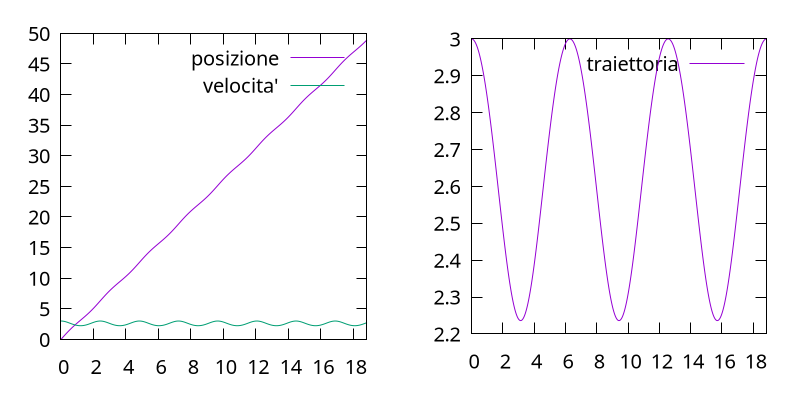
\includegraphics[width=1\textwidth]{real_oscillator_1_1.png}
		      \caption{Oscillatore ideale imperturbato $(\theta(0)=0, \dot{\theta}(0)=3)$, nel caso non in equilibro.}
		      \labfig{real_oscil_1_1}
	      \end{figure}

	      Come si puo' osservare lo spazio delle fasi e' composto principalmente da due
	      casi di traiettorie: la prima in \reffig{real_oscil_1} corrisponde ad un ellisse; mentre, se l'energia cinetica supera l'energia potenziale di carattere oscillatoria, si osserva il caso non in equilibrio: al di sopra e al di sotto delle possibili traiettorie ellissoidali si ottengono traiettorie sinusoidali come in \reffig{real_oscil_1_1}. I risultati corrispondono correttamete con la teoria.

	\item Nel caso dell'oscillatore smorzato si ottengono i seguenti risultati:

	      \begin{figure} [H]
		      \centering
		      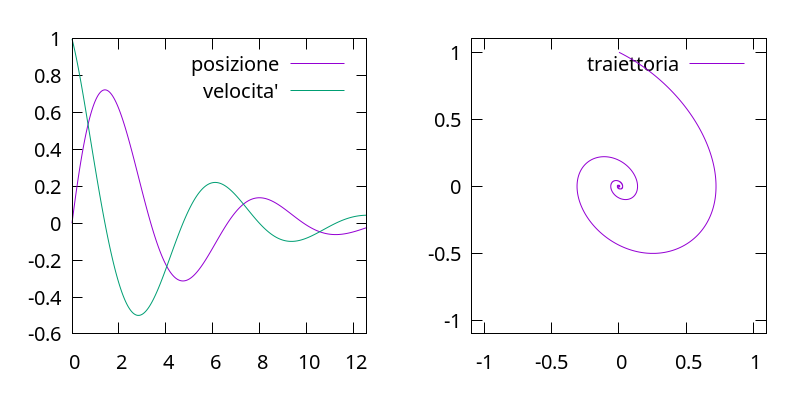
\includegraphics[width=1\textwidth]{real_oscillator_2_0.5.png}
		      \caption{Oscillatore ideale smorzato $(\theta(0)=0, \dot{\theta}(0)=1)$, nel caso $\gamma=0.5$.}
		      \labfig{real_oscil_2_0.5}
	      \end{figure}

	      \begin{figure} [H]
		      \centering
		      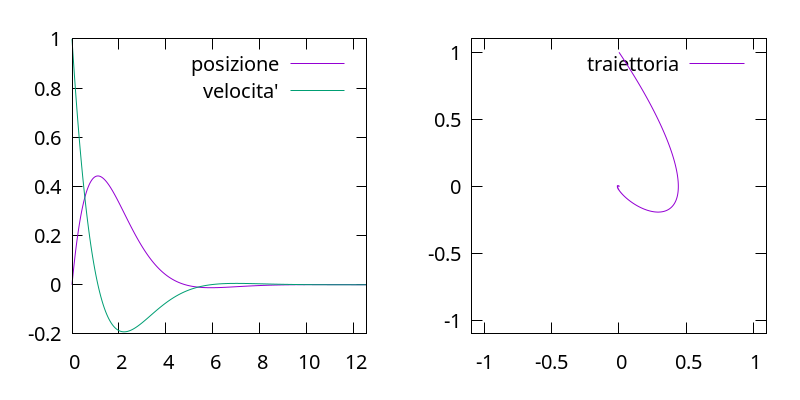
\includegraphics[width=1\textwidth]{real_oscillator_2_1.5.png}
		      \caption{Oscillatore ideale imperturbato $(\theta(0)=0, \dot{\theta}(0)=1)$, nel caso $\gamma=1.5$.}
		      \labfig{real_oscil_2_1.5}
	      \end{figure}

	      Si osserva in questo caso che il termine di smorzamento influenza la traiettoria delle oscillazioni, in particolare, per $\gamma=0.5$ si osserva un'oscillazione smorzata, mentre per $\gamma=1.5$ si osserva un'oscillazione smorzata simil-critica. Lo spazio delle fasi assume una traiettoria a spirale: la spiegazione fisica e' molto semplice, lo smorzamento porta ad un continuo rallentamento del sistema che e' destinato (qualsiasi siano i valori iniziali) a convergere ad un punto. Per questa ragione non vengono inclusi casi di valori iniziali differenti poiche' si otterra' sempre un carattere oscillatorio iniziale per sistemi inizialmente non stabili ma che cadranno necessariamente in una spirale simile alle sovracitate.

	\item Si studia,infine, il caso di smorzamento forzato:

	      \begin{figure} [H]
		      \centering
		      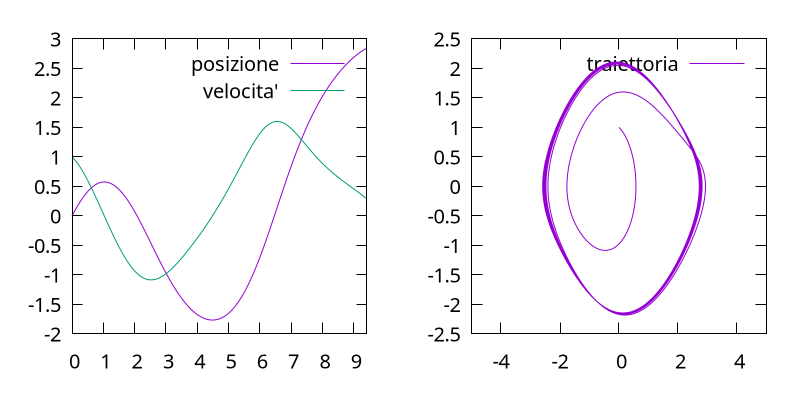
\includegraphics[width=1\textwidth]{real_oscillator_3_0.5_0.5.png}
		      \caption{Oscillatore forzato $(\theta(0)=0, \dot{\theta}(0)=1)$, nel caso $\gamma=0.5, A=0.5$.}
		      \labfig{real_oscil_3_0.5}
	      \end{figure}

	      \begin{figure} [H]
		      \centering
		      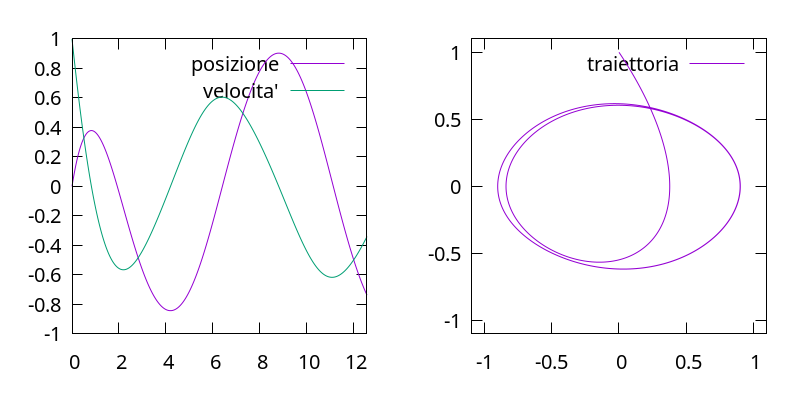
\includegraphics[width=1\textwidth]{real_oscillator_3_1.5_1.5.png}
		      \caption{Oscillatore forzato $(\theta(0)=0, \dot{\theta}(0)=1)$, nel caso $\gamma=1.5, A=1.5$.}
		      \labfig{real_oscil_3_1.5}
	      \end{figure}

	      In \reffig{real_oscil_3_0.5} e in \reffig{real_oscil_3_1.5} si evince chiaramente l'effetto del termine forzante: la traiettoria inizialmente a spirale si dilata e torna ad un caso ellissoide coerentemente con il caso in equilibrio imperturbato. La forzante, il termine $A$, definisce la nuova ampiezza di oscillazione stabile, mentre il termine $\gamma$ definisce la velocità di convergenza al nuovo equilibrio.



\end{enumerate}



\subsection{Attrattore di Lorenz}

\paragraph{Richiesta}

Studiare il sistema di ODE:

\begin{equation}
	\begin{cases}
		\dot{x}(t) = 10(y(t) - x(t))       \\
		\dot{y}(t) = 28x(t) - y(t) - xz(t) \\
		\dot{z}(t) = -8/3 z(t) + xy(t)
	\end{cases}
\end{equation}

\begin{enumerate}
	\item Utilizzare il metodo di Eulero, il metodo di Runge-Kutta del secondo ordine (RK2) e il metodo di Runge-Kutta del quarto ordine (RK4).
	\item Tracciare il grafico di $(x, y)$, $(x, z)$ e $(y, z)$.
\end{enumerate}

\paragraph{Implementazione}

\subparagraph{File necessari} \texttt{lorenz.cpp}

L'implementazione del sistema di equazioni differenziali è immediata essendo gia'
al primo ordine.

\paragraph{Osservazioni e analisi risultati}

Considerando un passo $\Delta t = 0.01$, un intervallo di tempo $t \in [0, 10]$ e valori iniziali $\vec{r}(0)=(0,0,0), \dot{r}(0)=(1,1,1)$ si ottengono le seguenti sezioni della soluzione:

\begin{figure} [H]
	\centering
	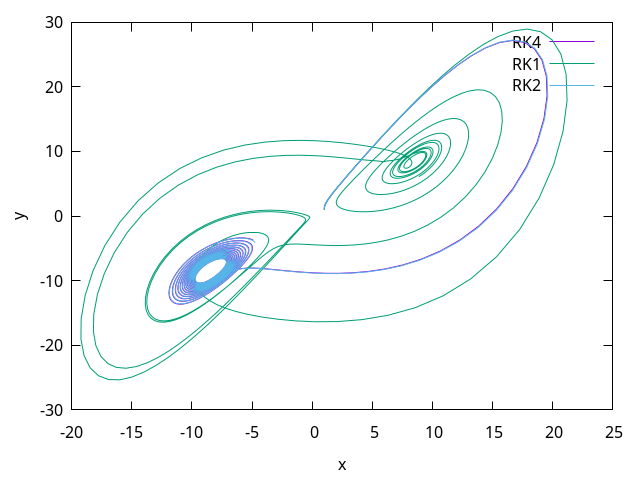
\includegraphics[width=1\textwidth]{lorenz_x_y.png}
	\labfig{real_oscil_3_1.5}
\end{figure}

\begin{figure} [H]
	\centering
	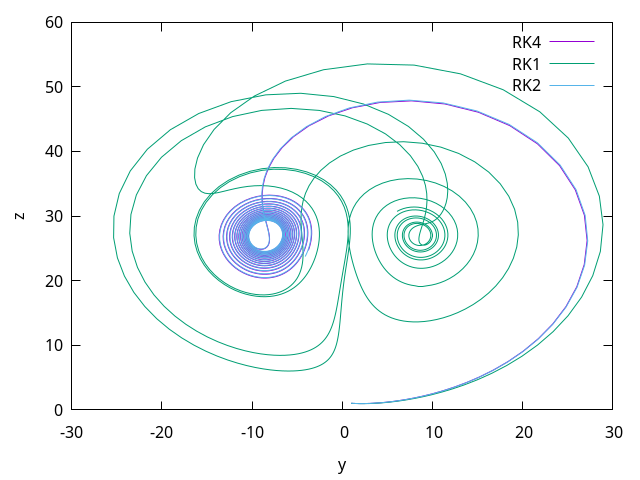
\includegraphics[width=1\textwidth]{lorenz_y_z.png}
	\labfig{real_oscil_3_1.5}
\end{figure}

\begin{figure} [H]
	\centering
	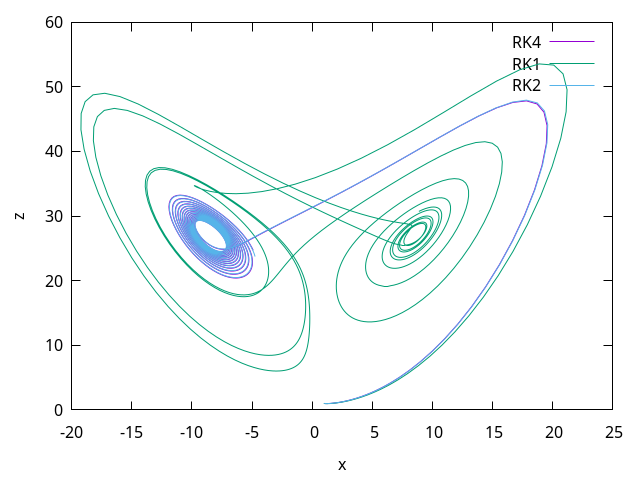
\includegraphics[width=1\textwidth]{lorenz_x_z.png}
	\labfig{real_oscil_3_1.5}
\end{figure}

Il risultato ottenuto e' il noto \textit{Attrattore di Lorenz}, e' inoltre risaputo dalla teoria che il sistema di equazioni differenziali descritto sia caotico: piccole variazioni nei valori iniziali portano a grandi variazioni nel sistema, come si puo' notare dai grafici ottenuti, infatti la differenza dell'ordine del metodo (sopratutto nel metodo di Eulero) porta una variazione considerevole nello step successivo che porta quindi ad un risultato considerevolmente diverso dato un intervallo di tempo adeguato rispetto al differenza tra gli ordine dei metodi considerati. Inoltre, si osserva che il sistema e' invariante per rotazioni, infatti, le traiettorie ottenute sono simmetriche rispetto all'asse $z$.


\subsection{Sistema a tre corpi}

\paragraph{Richiesta}

Studiare il sistema gravitazionale che obbedisce alle equazioni del moto:

\begin{equation}
	\ddot{\vec{x}}_i = \sum_{j \neq i} m_j \; \frac{ \vec{x}_j - \vec{x}_i}{|\vec{x}_j - \vec{x}_i|^3}
	\label{eq:3body}
\end{equation}

Nel caso di tre masse puntiformi, $i = 1, 2, 3$, con i seguenti parametri e condizioni iniziali:

\begin{itemize}
	\item
	      \quad\parbox{\linewidth}{
		      \begin{math}
			      m_1 = m_2 = m_3 = 1 \\
			      \vec{x}_1 = (1, 0, 0), \quad \dot{\vec{x}}_1 = (0, 0.15, -0.15) \\
			      \vec{x}_1 = (-1, 0, 0), \quad \dot{\vec{x}}_1 = (0, -0.15, 0.15) \\
			      \vec{x}_1 = (0, 0, 0), \quad \dot{\vec{x}}_1 = (0, 0, 0)
		      \end{math}
		      \\
	      }
	\item
	      \quad\parbox{\linewidth}{
		      \begin{math}
			      m_1 = 1.6, m_2 = m_3 = 0.4 \\
			      \vec{x}_1 = (1, 0, 0), \quad \dot{\vec{x}}_1 = (0, 0.4, 0) \\
			      \vec{x}_1 = (-1, 0, 0), \quad \dot{\vec{x}}_1 = (0, -0.8, 0.7) \\
			      \vec{x}_1 = (0, 0, 0), \quad \dot{\vec{x}}_1 = (0, -0.8, -0.7)
		      \end{math}
	      }
\end{itemize}

\begin{enumerate}
	\item Risolvere numericamente il sistema di equazioni.
	\item Tracciare il grafico dell'energia totale del sistema in funzione del tempo.
\end{enumerate}

\paragraph{Implementazione}

\subparagraph{File necessari} \texttt{gravitation.cpp}

Nella matrice della soluzione si sceglie di ordinare la soluzione ad ogni time step nel seguente modo:

\[
	\begin{pmatrix}
		r_{1,x}(t_0) & r_{1,y}(t_0) & \dots & r_{3,z}(t_0) & v_{1,x}(t_0) & \dots & v_{3,z}(t_0) \\
		\vdots                                                                                   \\

		r_{1,x}(t_n) & r_{1,y}(t_n) & \dots & r_{3,z}(t_n) & v_{1,x}(t_n) & \dots & v_{3,z}(t_n) \\
	\end{pmatrix}
\]

La funzione che definisce il sistema dovra' quindi tradurre l'equazione \ref{eq:3body} in un sistema di equazioni differenziali al primo ordine che rispettino l'ordine della matrice:

\begin{lstlisting} [language=C++]
...
  // Calcoliamo la accelerazione di interazione per ogni corpo
  auto grav_accell = [&](int i, int j) -> tensor::Tensor<double> {
    auto r_ij = tensor::Tensor<double>::Vector(3);
    for (int k = 0; k < 3; k++) {
      // Utilizziamo l'ordine specificato nella matrice
      r_ij(k) = y(3 * i + k) - y(3 * j + k);
    }

    double dist = r_ij.Norm();
    double dist_cubed = std::pow(dist, 3);

    auto accell = tensor::Tensor<double>::Vector(3);

    for (int k = 0; k < 3; ++k) {
      accell(k) = -masses(j) * r_ij(k) / dist_cubed;
    }

    return accell;
  };

  for (int i = 0; i < 3; ++i) {
    for (int k = 0; k < 3; ++k) {
      // Vengono aggiornate le posizioni
      dydt(3 * i + k) = y(3 * (i + 3) + k);
    }

    auto acc = tensor::Tensor<double>::Vector(3);
    // Utilizzando modulo 3 si riottengono gli indici delle posizioni 
    // dei corpi e calcoliamo l'accelerazione
    auto acc1 = grav_accell(i, (i + 1) % 3);
    auto acc2 = grav_accell(i, (i + 2) % 3);

    for (int k = 0; k < 3; ++k) {
      // Si aggiornano le velocita'
      dydt(3 * (i + 3) + k) = (acc1 + acc2)(k);
    }
  }
\end{lstlisting}

Si ottiene dunque la nuova riga della matrice dal vettore riga \texttt{dydt} allo step successivo.



\paragraph{Osservazioni e analisi risultati}

Utilizzando il metodo $RK4$ e step $\Delta t = 0.01$ si ottengono i seguenti risultati:

\begin{enumerate}
	\item
	      \begin{marginfigure}
		      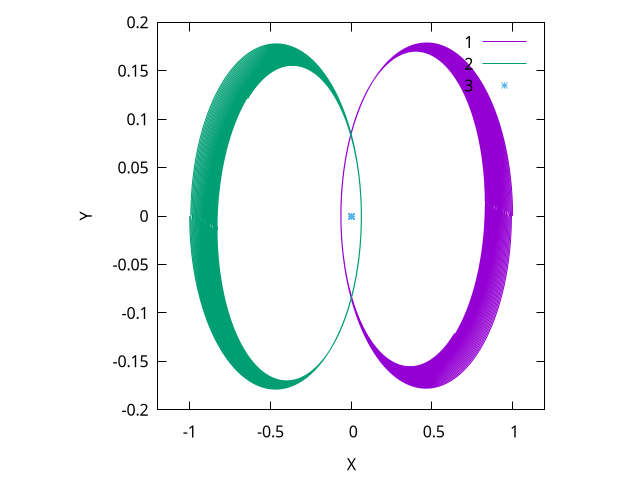
\includegraphics[width=1.5\textwidth]{gravitation_1_xy.png}
		      \caption{Sezione sul piano XY del primo punto}
		      \labfig{grav_1}
	      \end{marginfigure}

	      \begin{marginfigure}
		      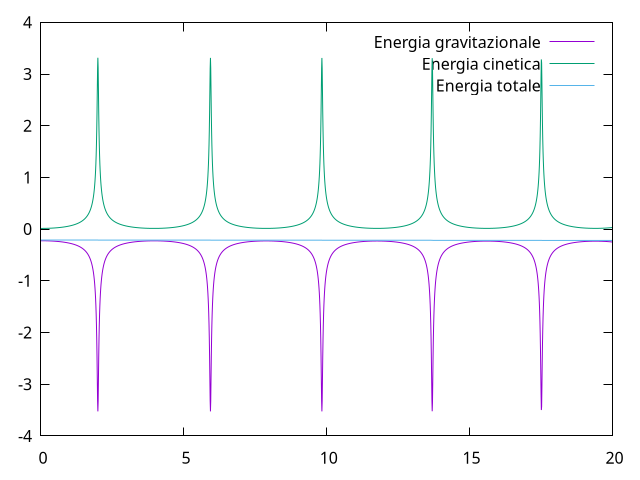
\includegraphics[width=1.5\textwidth]{grav_energy_1.png}
		      \caption{Grafico delle energie per il punto 1}
		      \labfig{grav_energy_1}
	      \end{marginfigure}

	      Dalle figure \reffig{grav_1} e \reffig{grav_energy_1} si osserva che, data la simmetria dei dati iniziali, la traiettoria dei corpi e' simmetrica rispetto all'asse $x$. Inoltre, si osserva che l'energia totale del sistema e' conservata, come ci si aspetta dal sistema gravitazionale, per valori non troppo grandi di $t$, piu' aumenta il tempo piu' il trend dell'energia totale diminuisce seguendo una retta di pendenza negativa, l'approssimazione del metodo $RK4$ dissipa energia per valori grandi di $t$; si conferma, inoltre, la presenza di un sistema legato data la presenza di una energia totale negativa.


	\item
	      \begin{marginfigure}
		      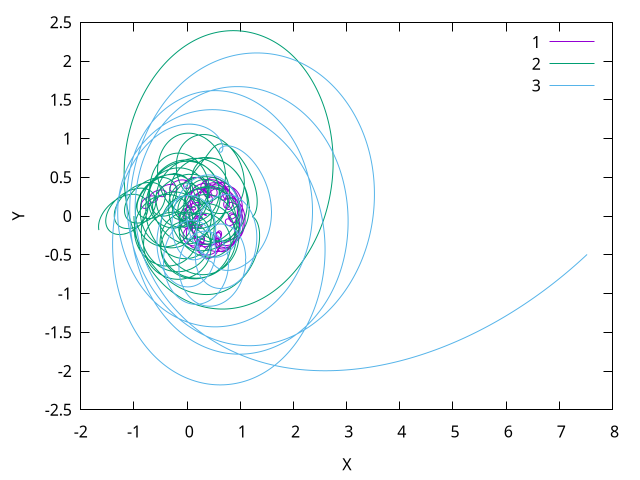
\includegraphics[width=1.5\textwidth]{gravitation_2_xy.png}
		      \caption{Sezione sul piano XY del primo punto}
		      \labfig{grav_2}
	      \end{marginfigure}

	      \begin{marginfigure}
		      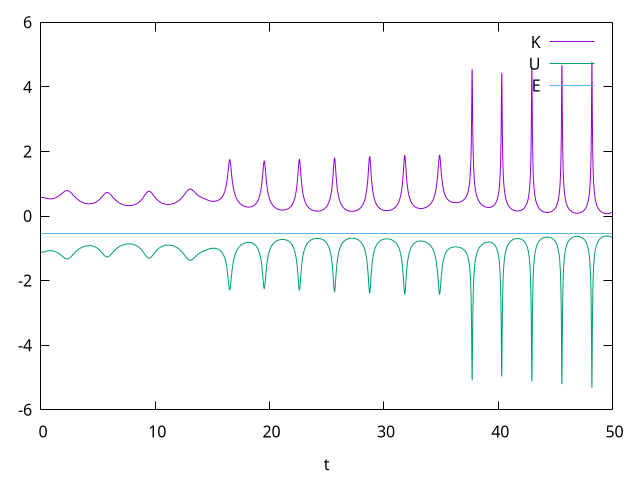
\includegraphics[width=1.5\textwidth]{grav_energy_2.png}
		      \caption{Grafico delle energie per il punto 2}
		      \labfig{grav_energy_2}
	      \end{marginfigure}

	      % Stesso trend negativo per le energie, il sistema e' in questo caso instabile 

        Nei grafici \reffig{grav_2} e \reffig{grav_energy_2} si osserva che il sistema e' caotico e legato. Si ripresenta nuovamente la pendenza negativa dell'energia totale seppure con un coefficiente relativamente basso non apprezabile a queste scale.


\paragraph{Conclusioni}

I metodi Runge-Kutta utilizzati negli esercizi non garantiscono la conservazione dell'energia del sistema: quando i corpi si avvicinano molto tra di loro si perdono molte informazioni sul sistema, quest'ultime e l'intervallo di step utilizzato non sono adeguatamente distribuiti rispetto alla forza esercitata tra i due corpi nello step corrente. Utilizzando degli intervalli di tempo in funzione della distanza tra i corpi si otterrebbero misure piu' precise, utilizzando, come nel seguente esercizio, uno step fisso nel calcolo si perdono informazioni quando i corpi sono piu' vicini e quindi molto piu' veloci. Oltre a questa soluzione personalmente ipotizzata si possono utilizzare metodi che garantiscono la conservazione di dell'energia: i \textit{Metodi Simplettici} 

%TODO: citare metodi simplettici







\end{enumerate}









